
\section{The OS Project Components}\label{section:projectcomponents}

The directories in the  project root  are outlined in Figure~\ref{figure:osprojectrootdir}.

If you download the OS package, you get these additional COIN-OR projects. The links to the project home pages are provided below and give more information on these projects.
\begin{itemize}
\item {\tt Bonmin}\index{COIN-OR projects!Bonmin@{\tt Bonmin}} - {\tt\UrlBonmin}
\item {\tt BuildTools}\index{COIN-OR projects!BuildTools@{\tt BuildTools}} - {\tt\UrlBuildtools}
\item {\tt Cbc}\index{COIN-OR projects!Cbc@{\tt Cbc}} - {\tt\UrlCbc}
\item {\tt Cgl}\index{COIN-OR projects!Cgl@{\tt Cgl}} - {\tt\UrlCgl}
\item {\tt Clp}\index{COIN-OR projects!Clp@{\tt Clp}} - {\tt\UrlClp}
\item {\tt CoinUtils}\index{COIN-OR projects!CoinUtils@{\tt CoinUtils}} - {\tt\UrlCoinUtils}
\item {\tt Couenne}\index{COIN-OR projects!Couenne@{\tt Couenne}} - {\tt\UrlCouenne}
\item {\tt CppAD}\index{COIN-OR projects!CppAD@{\tt CppAD}} - {\tt\UrlCppad}
\item {\tt DyLP}\index{COIN-OR projects!DyLP@{\tt DyLP}}  - {\tt\UrlDylp}
\item {\tt Ipopt}\index{COIN-OR projects!Ipopt@{\tt Ipopt}} - {\tt\UrlIpopt}
\item {\tt Osi}\index{COIN-OR projects!Osi@{\tt Osi}} - {\tt\UrlOsi}
\item {\tt SYMPHONY}\index{COIN-OR projects!SYMPHONY@{\tt SYMPHONY}}   - {\tt\UrlSymphony}
\item {\tt Vol}\index{COIN-OR projects!Vol@{\tt Vol}} - {\tt\UrlVol}
\end{itemize}

The following directories are also in the project root.
\begin{itemize}
\item {\tt bin} - after executing {\tt make install}\index{make install@{\tt make install}}
the bin directory will contain {\tt OSSolverService}\index{OSSolverService@{\tt OSSolverService}}, {\tt clp}, {\tt cbc}  
and {\tt symphony}.

\item {\tt Data} - this directory contains numerous test problems that are used by the unit tests of
the COIN-OR projects just mentioned.

\item {\tt doxydoc} - is a folder for documentation.

\item {\tt include} - is a directory for header files. If the user wishes to write code to link against any of the libraries in the {\tt lib} directory, it may be necessary to include these header files.

\item {\tt lib} - is a directory of libraries. After running {\tt make install} the OS library along with all other COIN-OR libraries are installed in {\tt lib}.

\item {\tt ThirdParty} - is a  directory for third-party software. For example, if AMPL\index{AMPL} related software
such as {\tt OSAmplClient}\index{OSAmplClient@{\tt OSAmplClient}} is used, then certain AMPL libraries need to be present.
This should go into the {\tt ASL} directory in {\tt ThirdParty.}
\end{itemize}


The directories in the OS directory are outlined in Figure~\ref{figure:osdirectory}.  The OS directories include the following:


\begin{figure}
\centering
%\includegraphics[scale=0.8]{\figurepath/OSDirectory.png}
\includegraphics[scale=0.8]{./figures/OSDirectory.png}
\caption{The OS directory.}
\label{figure:osdirectory}
\end{figure}



\begin{itemize}


\item {\tt applications} - is a directory that holds  the 
{\tt OSAmplClient}\index{OSAmplClient@{\tt OSAmplClient}}
and {\tt OSFileUpload}  applications in subdirectories called, respectively, {\tt amplClient} and {\tt fileUpload}.
See Section \ref{section:amplclient} and~\ref{section:fileupload}.

\item {\tt data} - is a directory that holds test problems. These test problems are used by the
{\tt unitTest}\index{unitTest@{\tt unitTest}} of the OS Project. Many of these files are also used to illustrate
how the {\tt OSSolverService}\index{OSSolverService@{\tt OSSolverService}} works.
See Section~\ref{section:ossolverservice}.

\item {\tt doc} - is the directory with documentation, including this {\it OS User's Manual}.

\item {\tt examples} - is a directory with code examples that illustrate various aspects of the OS project.
These are described in Section~\ref{section:examples}.

\item {\tt inc} - is the directory with the config\_os.h file which has information about which projects
are included in the distribution.

\item {\tt m4} - is a directory that  contains macro scripts written in the m4 language for auto configuration.

\item {\tt MSVisualStudio} - is a directory that  contains folders for the solution files for the
Microsoft Visual Studio\index{Microsoft Visual Studio} IDE.  The subdirectories are organized by the version
of Visual Studio. We currently provide solution files for versions 8 and~9.

\item {\tt schemas} - is the directory that contains the W3C XSD (see \url{www.w3.org}) schemas that are
behind the OS standards. These are described in more detail in Section~\ref{section:schemadescriptions}.

\item {\tt src} - is the directory with all of the source code for the OS Library and for the executable
{\tt OSSolverService}. The OS Library components are described in Section~\ref{section:oslibrary}.

\item {\tt stylesheets} - this directory contains the XSLT stylesheet that is used to transform the solution
instance in OSrL format into HTML so that it can be displayed in a browser.

\item {\tt test} - this directory contains the {\tt unitTest}.


\item  {\tt wsdl} - is a directory of WSDL (Web Services Discovery Language) files. These are used to specify
the inputs and outputs for the methods and other invocation details provided by a Web service. The most relevant
file for the current version of the OS project is {\tt OShL.wsdl}.
This describes the set of inputs and outputs for the methods implemented in the {\tt OSSolverService}.
See Section~\ref{section:ossolverservice}.

\end{itemize}

